%\documentclass[conference]{llncs}
\documentclass[runningheads]{llncs}
%\usepackage{minipage}
\usepackage[T1]{fontenc}
\usepackage[table]{xcolor}
\usepackage[english]{babel}
\usepackage[utf8]{inputenc}
\usepackage[style=numeric-comp]{biblatex}
\usepackage{amsmath}
\usepackage{amsfonts}
\addbibresource{./literature.bib}% Syntax for version >= 1.2
\usepackage{graphicx}
\graphicspath{{./images/}}
\usepackage{multirow}
\usepackage{enumitem}
\usepackage{tikz}
%\usepackage{amsthm}
\usepackage{rotating}

% circles
\usepackage{wasysym}
\newcommand{\Tdot}{$\CIRCLE$}
\newcommand{\Thdot}{$\LEFTcircle$}
\newcommand{\Twdot}{$\Circle$}

% for fancy table with rotated column titles
\usepackage{tabularx}
\usepackage{adjustbox}
\newcolumntype{R}[2]{%
    >{\adjustbox{angle=#1,lap=\width-(#2)}\bgroup}%
    l%
    <{\egroup}%
}
\newcommand*\rot{\multicolumn{1}{R{45}{0.01em}}}% no optional argument here, please!
\newcommand*\rota{\multicolumn{1}{R{90}{0.01em}}}% no optional argument here, please!
\def\hb{\hbox to 10.7 cm{}}

%colors in tables
\definecolor{abfred}{RGB}{255, 215, 215}
\definecolor{abf-rg-1}{RGB}{251,213,242}
\definecolor{abf-rg-2}{RGB}{243,212,249}
\definecolor{abf-rg-3}{RGB}{213,210,245}
\definecolor{abf-rg-4}{RGB}{208,231,242}
\definecolor{abf-rg-5}{RGB}{206,238,223}
\definecolor{abf-rg-6}{RGB}{205,236,210}
\definecolor{abf-rg-7}{RGB}{211,234,204}
\definecolor{abfgreen}{RGB}{221,232,203}
\definecolor{abforange}{RGB}{255, 245, 206}

%fix commands
\newcommand{\fixnote}[2]{\textbf{\color{red}{FIX}}\footnote{{\bf #1:} #2}}
\newcommand{\fix}[2]{{\color{red}{\bf tofix:} #2}}
\newcommand{\toremove}[2]{{\color{blue}{\bf toremove:} #2}}
% \renewcommand{\fixnote}[2]{}
% \renewcommand{\fix}[2]{}

\newcommand{\assertionRegion}{\mathcal{A}}
\newcommand{\beliefRegion}{\mathcal{B}}
\newcommand{\factRegion}{\mathcal{F}}
\newcommand{\rcc}{rcc}
\newcommand{\agentuniverse}{Ag}
\newcommand{\abf}{\assertionRegion,\beliefRegion,\factRegion}
\newcommand{\abftheory}{\assertionRegion\beliefRegion\factRegion}
\newcommand{\Rcc}[2]{rcc(#1,#2)}
\newcommand{\connects}[2]{C(#1,#2)}
\newcommand{\disconnected}[2]{\neg C(#1,#2)}
\newcommand{\partof}[2]{P(#1,#2)}
\newcommand{\overlaps}[2]{O(#1,#2)}
\newcommand{\eq}[2]{EQ(#1,#2)}
\newcommand{\pp}[2]{PP(#1,#2)}
\newcommand{\po}[2]{PO(#1,#2)}
\newcommand{\ppi}[2]{PPi(#1,#2)}
\newcommand{\dr}[2]{DR(#1,#2)}
\newcommand{\all}[2]{T(#1,#2)}
\newcommand{\rassert}[3]{\mathcal{A}_{#1\rightarrow #2}#3}
\newcommand{\lassert}[3]{\mathcal{A}_{#1\leftarrow #2}#3}

\newcommand*\halfbullet[1][0.4ex]{%
  \begin{tikzpicture}
	  \raisebox{0.6pt}{\draw[fill] (0,0)-- (90:#1) arc (90:270:#1) -- cycle ;
	  \draw (0,0) circle (#1);}
  \end{tikzpicture}}

\newcommand{\fakedmapsfromchar}{%
  \mathrel{\mathpalette\reflectmathchar\mapstochar}%
}
\makeatletter
\newcommand{\reflectmathchar}[2]{%
  \reflectbox{$\m@th#1#2$}%
}
\makeatother
\newcommand{\rightbararrow}{\rightarrow\fakedmapsfromchar}
\newcommand{\leftbararrow}{\mapstochar\rightarrow}
\newcommand{\rightleftbararrow}{\mapstochar\rightarrow\fakedmapsfromchar}
\setlength{\fboxrule}{0.1pt}
\setlength{\fboxsep}{1.5pt}
\newcommand{\secureportelem}{\mathrel{\rightarrow}}
\newcommand{\secureport}{\fbox{\ensuremath \secureportelem}}
\newcommand{\dropportelem}{\mathrel{\circ\!\!\rightarrow}}
\newcommand{\dropport}{\fbox{\ensuremath \dropportelem}}
\newcommand{\insertportelem}{\mathrel{\bullet\!\!\rightarrow}}
\newcommand{\insertport}{\fbox{\ensuremath \insertportelem}}
\newcommand{\injectionportelem}{\mathrel{\halfbullet\!\!\rightarrow}}
\newcommand{\injectionport}{\fbox{\ensuremath \injectionportelem}}
\newcommand{\selectiveportelem}{\mathrel{\leftbararrow}}
\newcommand{\selectiveport}{\fbox{\ensuremath \selectiveportelem}}
\newcommand{\selectiveinsertportelem}{\mathrel{\bullet\!\!\leftbararrow}}
\newcommand{\selectiveinsertport}{\fbox{\ensuremath \selectiveinsertportelem}}
\newcommand{\selectiveinjectionportelem}{\mathrel{\halfbullet\!\leftbararrow}}
\newcommand{\selectiveinjectionport}{\fbox{\ensuremath \selectiveinjectionportelem}}
\newcommand{\selectivedropportelem}{\mathrel{\circ\!\!\leftbararrow}}
\newcommand{\selectivedropport}{\fbox{\ensuremath \selectivedropportelem}}
%communication channels
%secure input port
\newcommand{\sdcom}{\mathrel{\rightarrow\!\!\circ}}
\newcommand{\sicom}{\mathrel{\rightarrow\!\!\bullet}}
\newcommand{\sjcom}{\mathrel{\rightarrow\!\!\halfbullet}}
\newcommand{\ssdcom}{\mathrel{\rightbararrow\!\!\circ}}
\newcommand{\ssicom}{\mathrel{\rightbararrow\!\!\bullet}}
\newcommand{\ssjcom}{\mathrel{\rightbararrow\!\halfbullet}}
%drop input port
\newcommand{\ddcom}{\mathrel{\circ\!\!\rightarrow\!\!\circ}}
\newcommand{\dicom}{\mathrel{\circ\!\!\rightarrow\!\!\bullet}}
\newcommand{\dscom}{\mathrel{\circ\!\!\rightarrow}}
%insert input port
\newcommand{\idcom}{\mathrel{\bullet\!\!\rightarrow\!\!\circ}}
\newcommand{\iicom}{\mathrel{\bullet\!\!\rightarrow\!\!\bullet}}
\newcommand{\ijcom}{\mathrel{\bullet\!\!\rightarrow\!\!\halfbullet}}
\newcommand{\isdcom}{\mathrel{\bullet\!\!\rightbararrow\!\!\circ}}
\newcommand{\isicom}{\mathrel{\bullet\!\!\rightbararrow\!\!\bullet}}
\newcommand{\isjcom}{\mathrel{\bullet\!\!\rightbararrow\!\halfbullet}}
\newcommand{\iscom}{\mathrel{\bullet\!\!\rightarrow}}
%injection input
\newcommand{\jdcom}{\mathrel{\halfbullet\!\!\rightarrow\!\!\circ}}
\newcommand{\jicom}{\mathrel{\halfbullet\!\!\rightarrow\!\!\bullet}}
\newcommand{\jjcom}{\mathrel{\halfbullet\!\!\rightarrow\!\!\halfbullet}}
\newcommand{\jsdcom}{\mathrel{\halfbullet\!\!\rightbararrow\!\!\circ}}
\newcommand{\jsicom}{\mathrel{\halfbullet\!\!\rightbararrow\!\!\bullet}}
\newcommand{\jsjcom}{\mathrel{\halfbullet\!\!\rightbararrow\!\halfbullet}}
\newcommand{\jscom}{\mathrel{\halfbullet\!\!\rightarrow}}
%selective drop input
\newcommand{\sddcom}{\mathrel{\circ\!\!\leftbararrow\!\!\circ}}
\newcommand{\sdicom}{\mathrel{\circ\!\!\leftbararrow\!\!\bullet}}
\newcommand{\sdjcom}{\mathrel{\circ\!\!\leftbararrow\!\!\halfbullet}}
\newcommand{\sdsdcom}{\mathrel{\circ\!\!\rightleftbararrow\!\!\circ}}
\newcommand{\sdsicom}{\mathrel{\circ\!\!\rightleftbararrow\!\!\bullet}}
\newcommand{\sdsjcom}{\mathrel{\circ\!\!\rightleftbararrow\!\halfbullet}}
\newcommand{\sdscom}{\mathrel{\circ\!\!\leftbararrow}}
%selective insertion
\newcommand{\sidcom}{\mathrel{\bullet\!\!\leftbararrow\!\!\circ}}
\newcommand{\siicom}{\mathrel{\bullet\!\!\leftbararrow\!\!\bullet}}
\newcommand{\sijcom}{\mathrel{\bullet\!\!\leftbararrow\!\!\halfbullet}}
\newcommand{\sisdcom}{\mathrel{\bullet\!\!\rightleftbararrow\!\!\circ}}
\newcommand{\sisicom}{\mathrel{\bullet\!\!\rightleftbararrow\!\!\bullet}}
\newcommand{\sisjcom}{\mathrel{\bullet\!\!\rightleftbararrow\!\halfbullet}}
\newcommand{\siscom}{\mathrel{\bullet\!\!\leftbararrow}}
%selective injection
\newcommand{\sjdcom}{\mathrel{\halfbullet\!\!\leftbararrow\!\!\circ}}
\newcommand{\sjicom}{\mathrel{\halfbullet\!\!\leftbararrow\!\!\bullet}}
\newcommand{\sjjcom}{\mathrel{\halfbullet\!\!\leftbararrow\!\!\halfbullet}}
\newcommand{\sjsdcom}{\mathrel{\halfbullet\!\!\rightleftbararrow\!\!\circ}}
\newcommand{\sjsicom}{\mathrel{\halfbullet\!\!\rightleftbararrow\!\!\bullet}}
\newcommand{\sjsjcom}{\mathrel{\halfbullet\!\!\rightleftbararrow\!\halfbullet}}
\newcommand{\sjscom}{\mathrel{\halfbullet\!\!\leftbararrow}}


%\newtheorem{definition}{Definition}%[section]
\newtheorem{hypothesis}{Hypothesis}%[section]
%\newtheorem{theorem}{Theorem}%[section]

\newcolumntype{C}[1]{>{\centering\let\newline\\\arraybackslash\hspace{0pt}}m{#1}}

\newcommand{\ON}[1]{\footnote{\textcolor{blue}{[[Oliviero: #1]]}}}

\begin{document}
\title{The Etiology of Cybersecurity}

\author{Michele Ambrosi, Francesco Beltramini, Federico De Meo,
 Oliviero Nardi, Mattia Pacchin, and Marco Rocchetto}

\authorrunning{Ambrosi et al.}

\institute{V-Research, Verona, Italy\\email: knowledgezero@v-research.it}
\maketitle

\begin{abstract}
	The objective of this research is to lay the foundations for the
	development of a scientific theory that determines (all and only) the
	possible insecure and secure configurations of any abstract system to be used for the risk assessment of systems. We
	claim that cybersecurity weaknesses (i.e. errors) are at the beginning
	of the causality chain that leads to cybersecurity attacks.  We
	formulate a hypothesis that we
	use to predict the weaknesses in the architectural design of an
	system. Our
	hypothesis allows for the definition of a mathematical formula which
	describes the cybersecurity of a system.  We implemented a prototype
	cybersecurity risk assessment tool that, based on our hypothesis,
	predicts the weaknesses in a UML model of a (cyber-physical) system.
  \keywords{Risk Management, Cyber-Physical Systems, Risk Assessment, Security Framework}
\end{abstract}


\section{Introduction}\label{sec:intro}
A \emph{scientific theory} is an explanation of a phenomenon such that the
explanation follows the scientific method. The \emph{scientific method} is an
\emph{empirical} method that aims at mitigating potential fallacies in
theories.  Karl Popper famously argued (e.g. in \autocite{Popper1959logic})
that a scientific theory can never be verified but only falsified, that a
theory should not be conceived by using the principle of
induction,\footnote{Einstein to Popper: ``[...] and I think (like
you, by the way) that theory cannot be fabricated out of the results of
observation, but that it can only be invented.'' \autocite{Popper1959logic}}
and that empirical experiments should be considered as the only evidence to
support the non-falseness of a scientific theory. 
In \autocite{Herley2016unfalsifiability}, Cormac Herley explores what he calls
``an asymmetry in computer security'', which he defines as follows: ``Things
can be declared insecure by observation, but not the reverse. There is no
observation that allows us to declare an arbitrary system or technique
secure''. With security, Herley only focuses on cybersecurity (we also use
security and insecurity, in this paper, only to refer to cyber-insecurity and
cybersecurity) and his intuition is that there is no scientific theory that can
predict the cybersecurity of a system, nor a theory that can predict all
possible insecurities of a system (which, by negation, may be used as a theory
of cybersecurity).  Herley then uses this argument to show that ``claims that
any measure is necessary for security are empirically unfalsifiable''. 
The goal of this paper is to address this issue and to lay the foundations of a scientific cybersecurity
theory.  We consider the problem raised by Herley not confined to ``computer
security'' but rather we reason on any abstract system (so that our scientific
hypothesis\footnote{In the remainder of this paper, we will use the word
hypothesis to refer to ``scientific hypothesis'' as a proposed scientific
theory that has not gone through an extensive series of tests. We
use ``logical theory'' to refer to a set of formal logical axioms.} may
be tested in any sound implementation such as a network, a mechanical, cyber, or
cyber-physical system, or even a single computer or a single device such as a
hard-drive).  
Instead of starting from reasoning about what makes a system secure or insecure,
we reason about what causes insecurities. 
We focus on insecurities only caused by
the exploitation of cybersecurity attacks, and we assume that achieving
cybersecurity means preventing all those attacks from being exploitable or
exploited.  Our hypothesis is that \emph{cybersecurity attacks are only caused by the
presence of errors in the design or implementation of a system} (i.e.
cybersecurity weaknesses).
With our approach, a list of weaknesses emerges from the mathematical
formulation of a system in a framework called $\abftheory$ (as in Assertions,
Beliefs, Facts in \autocite{Santaca2016abf})\footnote{Intuitively, as we will
see later, assertions correspond to an exchange of
information between agents, beliefs to internal
information considered true by the agent, and facts to
requirements.} predicts 4 main classes of weaknesses. Those classes are used to
calculate all the insecurity configurations of all the components of a system,
obtaining a precise estimation of all potential cybersecurity-related risks in
any given system. Our hypothesis can be falsified by means of experiments,
testing if all the predicted weaknesses are present in the system under consideration,
or testing if other (not predicted by our hypothesis) weaknesses are present.
In fact, if any cybersecurity weaknesses were to be found in a system and not
predicted by our hypothesis, the hypothesis could be declared incomplete.  If a
cybersecurity weakness would be predicted by our hypothesis but found to be impossible
to realize, our hypothesis could be declared as wrong.

\section{Literature Review}\label{sec:literature}

Cybersecurity attacks seem to be related to the creativity of the attacker
and thus unpredictable. 
Currently, the most complete understanding of insecurity issues is stored into
a network of databases of weaknesses (e.g.
CWE \autocite{MITRE2020CWEresearch}), vulnerabilities (e.g. CVE \autocite{CVE},
NVD \autocite{NIST2020NVD}), and attacks (e.g. CAPEC \autocite{MITRE2020CAPEC},
ATT\&CK \autocite{MITRE2020ATTACK}).  Those insecurity issues can be related to
the violation of one or more requirements (explicit or implicit) in the
specification, design or implementation of a system. The correlation 
between insecurity flaws and cybersecurity requirements has been used to define
standards such as the IEC 62443-1-3 (the Industrial communication networks -
Network and system security -- Part 3-3: System security requirements and
security levels) which defines requirements as ``confidentiality of information
in transit/at-rest''. More generally, the idea of defining cybersecurity requirements
as properties of a system was initially defined in 1970s with the 
CIA triad (Confidentiality, Integrity, Availability) and refined 
over the decades introducing related concepts such as authenticity or
non-repudiation, or introducing new ones such as ``responsibility'' in the
RITE approach (see \autocite{Samonas2014cia} for an overview of the evolution of the CIA triad).
The link between cybersecurity requirements and vulnerabilities is reported 
in the NVD databases by the CVSS \autocite{Mell2007CVSS} scoring system.
The CVSS evaluates of the severity of a vulnerability
by means of different metrics (such as attack complexity and user interaction)
and quantitatively evaluates the impact on the CIA triad.
While cybersecurity requirements, weaknesses, vulnerabilities, and attacks
have been extensively studied and implemented both in academia and industry
to provide tools for the testing or verification of systems, 
no scientific falsifiable theory correlates
cybersecurity requirements to necessary and sufficient conditions (e.g. mitigations) 
to declare a system secure \autocite{Herley2016unfalsifiability}.
Nonetheless, the extensive body of literature has scientific foundations,
for example, providing formal frameworks for the verification of 
properties %either necessary or sufficient conditions
for cybersecurity.
As a driver for our argumentation, we start by reviewing the key concepts
in the cybersecurity domain.

\subsection{Terminology}
We provide a baseline for a definition of
the terms that structure our current understanding of cybersecurity.

\emph{Vulnerability}.
	As defined in \autocite{cnssi20104009}
	(and adopted in \autocite{nist2013800-53}), is a ``weakness in an
	information system, system security procedures, internal
	controls, or implementation that could be exploited by a threat
	source''.

\emph{Weakness}. The definition given by the MITRE in
	\autocite{MITRE2020CWEweakness} of weakness is: `` a type of
	mistake that, in proper conditions, could contribute to the
	introduction of vulnerabilities within that product. This term
	applies to mistakes regardless of whether they occur in
	implementation, design, or other phases of a product
	lifecycle.'' A vulnerability, such as those enumerated on the
	Common vulnerabilities and Exposures (CVE) List, is a mistake
	that can be directly used by an attacker to gain access to a
	system or network.  The definition is circular if we interpret
	the word ``error'' and ``mistake'' with the same semantics: a
	weakness is an error that leads to a vulnerability and a
	vulnerability is a mistake which, in turn, is a weakness. The
	only difference between a weakness and vulnerability seems to
	be that one can consider weakness as a ground term and state
	that a vulnerability is caused by a weakness.

\emph{Exploit} ``[\ldots]
	(from the English verb to exploit, meaning to use something to
	one’s own advantage) is a piece of software, a chunk of data,
	or a sequence of commands that takes advantage of a bug or
	vulnerability to cause unintended or unanticipated behavior to
	occur on computer software, hardware, or something electronic
	(usually computerized).'' \autocite{wiki-exploit}.

\emph{Attack}. As defined by the International Standard
	ISO/IEC 27000, is an ``attempt to destroy, expose, alter,
	disable, steal or gain unauthorized access to or make
	unauthorized use of an asset''; where an \emph{Asset} is
	``anything that has value to the organization''.
	We do not consider ethical hackers as attacking a system. 
	In fact, we consider the term \emph{hack} as
	non-malicious (as, e.g. in \autocite{Stallman2002hacker}).
  
\emph{Threat}. As defined in \autocite{cnssi20104009}, is ``Any
	circumstance or event with the potential to adversely impact
	organizational operations (including mission, functions, image,
	or reputation), organizational assets, individuals, other
	organizations, or the Nation through an information system via
	unauthorized access, destruction, disclosure, modification of
	information, and/or denial of service''.

\begin{figure}[t]
\begin{minipage}[t]{0.4\textwidth}
	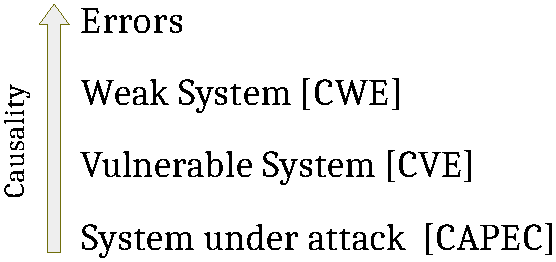
\includegraphics[width=\columnwidth]{causality.pdf}
\end{minipage}
\begin{minipage}[t]{0.6\textwidth}
	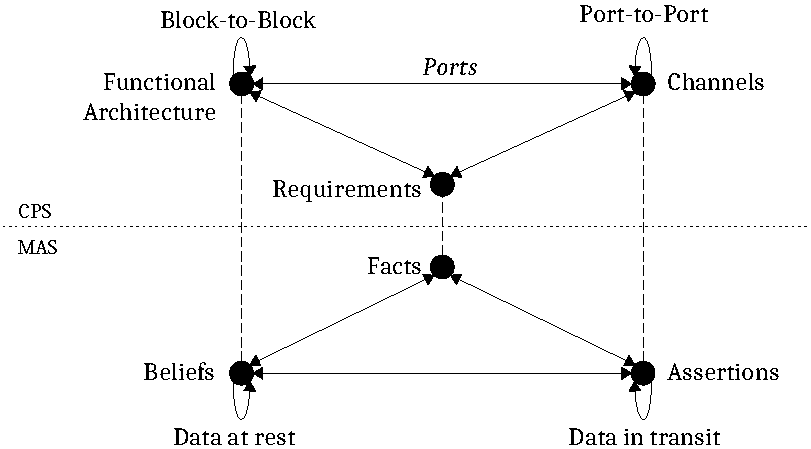
\includegraphics[width=.9\columnwidth]{abftheory.pdf}
\end{minipage}
  \caption{Etiology of cybersecurity (left). Mapping Epistemological Concepts to (Cyber-Physical) Systems Engineering (right).}
	\label{fig:causality}
	\label{fig:mashyp}
\end{figure}

As in Fig.~\ref{fig:causality}, in order to define a theory on cybersecurity we may
say that the presence of vulnerabilities is a necessary condition to
cause an attack in the system.  Those vulnerabilities are, in turn, caused by
the presence of weaknesses in the system.  Weaknesses are errors in the design
or implementation of a system and a theory on cybersecurity should
first predict the errors in a system design.

\section{A Cybersecurity Hypothesis in the $\abftheory$-framework}\label{sec:hypothesis}
To address the problem raised by Herley, we define how to
distinguish between a secure and an insecure system in the following steps 
of the engineering process:
\begin{enumerate}
  \item \emph{System Specification}: the \emph{functional} and \emph{physical requirements} are defined.
  \item \emph{Architecture Design}: the specification is structured into \emph{functional} and \emph{physical architectures}.
	\item \emph{Cybersecurity Risk Assessment}: potential \emph{weaknesses} (errors) and
		\emph{cybersecurity requirements} are identified.	
\end{enumerate}
We changed the focus from the attacker as the source of insecurity to the
potential design errors of a system. We now define a framework for the
definition of a system that we use to identify weaknesses as potential design
errors.

\subsection{Mereo-topological Reasoning}
\begin{table*}[t]
\centering
\begin{tabular}{cclll} 
\rota{\textbf{RCC3}}&\rota{\textbf{RCC5}}&\textbf{Terminology} & \textbf{Notation} & \textbf{Definition} \\
\hline
&&Connects with 			& $\mathit{C}(\mathit{X},\mathit{Y})$ 		& reflexive and symmetric \\
&&Disconnected from		& $\neg \mathit{C}(\mathit{X},\mathit{Y})$		& irreflexive or antisymmetric\\
&&Part of				& $\mathit{P}(\mathit{X},\mathit{Y})$		& $\forall \mathit{Z} ~\mathit{C}(\mathit{Z},\mathit{X}) \rightarrow \mathit{C}(\mathit{Z},\mathit{Y})$\\
&&Overlaps			& $\mathit{O}(\mathit{X},\mathit{Y})$		& $\exists \mathit{Z} ~\mathit{P}(\mathit{Z},\mathit{X})\wedge \mathit{P}(\mathit{Z},\mathit{Y})$\\
\Tdot&\Tdot& \textbf{Equal to} 		& $\mathit{EQ}(\mathit{X},\mathit{Y})$  		& $\mathit{P}(\mathit{X},\mathit{Y}) \wedge \mathit{P}(\mathit{Y},\mathit{X})$\\
\Tdot&&  \textbf{Overlaps Not Equal} 	& $\mathit{ONE}(\mathit{X},\mathit{Y})$		& $\mathit{O}(\mathit{X},\mathit{Y}) \land \neg \mathit{EQ}(\mathit{X},\mathit{Y})$ \\
\Tdot&\Tdot& \textbf{DiscRete from} 		& $\mathit{DR}(\mathit{X},\mathit{Y})$		& $\neg \mathit{O}(\mathit{X},\mathit{Y})$\\
&\Tdot&\textbf{Partial-Overlap}	& $\mathit{PO}(\mathit{X},\mathit{Y})$ 		& $\mathit{O}(\mathit{X},\mathit{Y})\wedge \neg \mathit{P}(\mathit{X},\mathit{Y}) \wedge \neg \mathit{P}(\mathit{Y},\mathit{X})$\\ 
&\Tdot&\textbf{Proper-Part-of} 	& $\mathit{PP}(\mathit{X},\mathit{Y})$ 		& $\mathit{P}(\mathit{X},\mathit{Y})\wedge \neg \mathit{P}(\mathit{Y},\mathit{X})$\\ 
	&\Tdot&\textbf{Proper-Part-of-\textit{\textbf{i}}nverse} & $\mathit{PPi}(\mathit{X},\mathit{Y})$ 		& $\mathit{P}(\mathit{Y},\mathit{X}) \wedge \neg \mathit{P}(\mathit{X},\mathit{Y})$\\
%&&\Tdot&\textbf{Externally Connected} 	& $\mathit{EC}(\mathit{X},\mathit{Y})$ 		& $\mathit{C}(\mathit{X},\mathit{Y}) \wedge \neg\mathit{O}(\mathit{X},\mathit{Y})$\\ 
%&&\Tdot&\textbf{Tangential PP} 	& $\mathit{TPP}(\mathit{X},\mathit{Y})$ 		& $\mathit{PP}(\mathit{X},\mathit{Y})\wedge\exists\mathit{Z}~[\mathit{EC}(\mathit{Z},\mathit{X}),\mathit{EC}(\mathit{Z},\mathit{Y})]$\\ 
%&&\Tdot&\textbf{Tangential PPi} 	& $\mathit{TPPi}(\mathit{X},\mathit{Y})$ 		& $\mathit{TPP}(\mathit{Y},\mathit{X})$\\ 
%&&\Tdot&\textbf{Non-Tangential PP} 	& $\mathit{NTPP}(\mathit{X},\mathit{Y})$ 		& $\mathit{PP}(\mathit{X},\mathit{Y})\wedge\neg\exists\mathit{Z}~[\mathit{EC}(\mathit{Z},\mathit{X}),\mathit{EC}(\mathit{Z},\mathit{Y})]$\\ 
%&&\Tdot&\textbf{Non-Tangential PPi} 	& $\mathit{NTPPi}(\mathit{X},\mathit{Y})$ 		& $\mathit{NTPP}(\mathit{Y},\mathit{X})$\\ 
\end{tabular}
\caption{RCC3 and RCC5 relations between regions $X$, $Y$ and $Z$ ~\label{tab:rcc358}~\label{tab:rcc}}
\end{table*}

Following \autocite{Santaca2016abf}, we define a system as a hierarchy of agents. Furthermore, we model an agent as a meronomy (an
hierarchy of part-whole relations) over the aforementioned constituents 
(assertions, beliefs, and facts), based on a standard definition of mereology
(i.e. based on the definition of parthood relation between \emph{parts}).  Due to
the necessity of considering different relations between parts (as we will show afterwards)
we extend the mereology to a
mereo-topology \autocite{Smith1996mereotopology,Varzi1994mereotopology,Rachavelpula2017mereotopology},
considering the relations in Tab.~\ref{tab:rcc358}.  For the sake of
readability, we use the term \emph{region} both to refer to a mereological part
and to a topological region.  Our aim is to create a meronomy (hierarchy of
part-whole relations) instead of the taxonomies (categorization based on
discrete sets) such as the one provided in \autocite{NIST2020NVD,CVE}
so that we don't need to rely on a scoring system (such as the CVSS) to assign
a quantitative evaluation of the cybersecurity of each entry. Instead, we want
a precise calculation of the number of insecure configurations of a system to
emerge from the mathematical formulation of our cybersecurity hypothesis.
A mereotopology, as defined in \autocite{Rachavelpula2017mereotopology},
is a mathematical structure where the basic relation between regions
is the reflexive and symmetric relation \emph{Connects With},
that we use to order a universe of agents
$\agentuniverse$ (see in Tab.~\ref{tab:rcc358}).  We use the Region Connection
Calculus (RCC), as defined in \autocite{bennettLogics,improvingRCC}, to provide
an axiomatization of the mereo-topological concepts. In its broader definition,
the RCC theory is composed by eight axioms, and is known as RCC8 \autocite{Grutter2008rcc}. Using
RCC5 instead of RCC8 prevents us from considering tangential connections
between spatial regions. However, tangential connections in RCC8 can be
considered as special cases of the more general spatial relations considered in
RCC5.
In Tab.~\ref{tab:rcc}, we summarize the axioms of the RCC (see, e.g., \autocite{Grutter2008rcc}).  We can now define a system
over the mereotopology using the RCC calculus, as follows, where $\rcc(X,Y)$ on
two generic regions $X,Y$ represents one of the possible RCC relations between
$X$ and $Y$. We note that all the RCC relations are symmetric with the exception
of those that have an explicit (related) inverse.

\begin{definition}{\bf System State --}\label{def:opsystem}
  A Cyber-Physical System (CPS), or a sub-system, state is defined as a tuple
	$s=\langle\rcc(\factRegion,\beliefRegion),\,\rcc(\factRegion,\assertionRegion),\,\rcc(\beliefRegion,\assertionRegion)\rangle$,
	where $\assertionRegion$,$\beliefRegion$, and $\factRegion$ are regions of
	assertions, beliefs (i.e. the beliefs generated by the behavior), and
	facts respectively, expressed as requirements.
\end{definition}

As in \autocite{Santaca2016abf}, it follows that, by defining
a system as a fixed number of regions, there exists
an upper-bound to the number of possible configuration of a system, defined by
the possible relations between the different regions.
The general formula to calculate the number of different types of agents is
$r^{\binom{n}{k}}$, where $r$ is the number of relations with arity $k$,
between $n$ different regions. In our case, $\binom{n}{k}=3$ since we consider $3$ regions 
($\assertionRegion$, $\beliefRegion$, and $\factRegion$), and all the relations
considered in the RCC are binary.  Hence, we have up to 125
different types of agents but only 54 of the 125 (as showed in
\autocite{improvingRCC}) combinations are topologically correct. 
For RCC5 there are $5^3=125$ theoretical combinations but
only 54 are correct with respect to the axioms.

In the quantitative evaluation of a single agent, as in Fig.~\ref{fig:quantitative},
we argue that only 1 configuration represents the nominal (expected) behavior 
of the agent while the other configurations are either impossible to 
implement or diverge from the intended nominal behavior. We note 
that the numbers reported here do not consider the details of the
engineering process and should be considered a limit of an abstract 
representation of the system.

\begin{figure}[t]
\begin{minipage}[t]{0.5\textwidth}
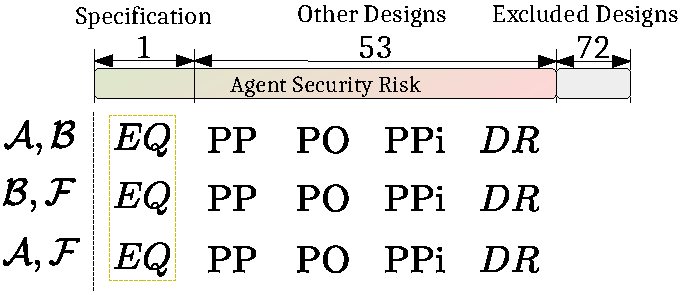
\includegraphics[width=.9\columnwidth]{quantitative.pdf}
\end{minipage}
\begin{minipage}[t]{0.5\textwidth}
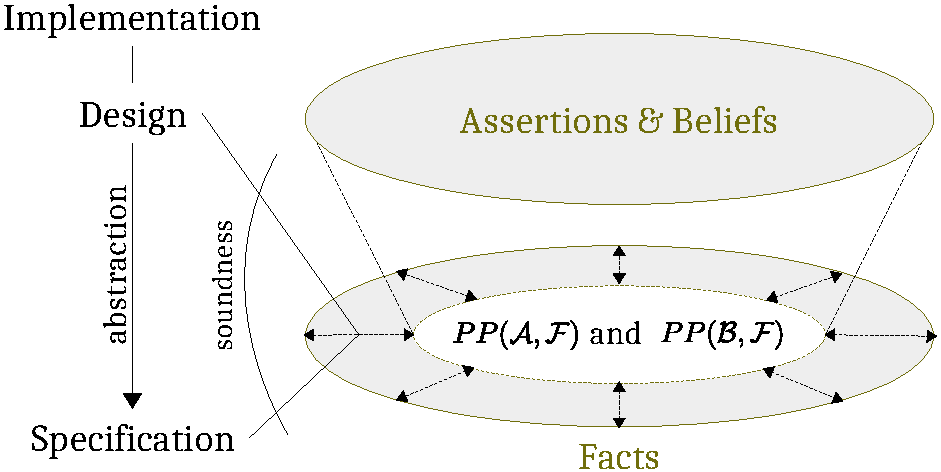
\includegraphics[width=.9\columnwidth]{soundness.pdf}
\end{minipage}
  \caption{Cybersecurity risk for a single agent (left). Example relation between facts, and assertions and beliefs (right).}
\label{fig:quantitative}
\label{fig:soundness}
\end{figure}

\subsection{Qualitative Evaluation of Agent Space in $\abf$}\label{sec:agentspace}
\begin{table}[t]
\centering
\begin{adjustbox}{width=.6\columnwidth}
\begin{tabular}{r||c|c|c|c|c} 
& \dr{$\assertionRegion$}{$\beliefRegion$} & 
	\po{$\assertionRegion$}{$\beliefRegion$}& 
	\pp{$\assertionRegion$}{$\beliefRegion$} &
	\ppi{$\assertionRegion$}{$\beliefRegion$} & 
	\eq{$\assertionRegion$}{$\beliefRegion$} \\
\hline
\hline %dr
 \multirow{3}{*}{\dr{$\beliefRegion$}{$\factRegion$}} & 
	\cellcolor{abfred} & %dr
	\cellcolor{abf-rg-1}\dr{$\assertionRegion$}{$\factRegion$} & %po
	\cellcolor{abf-rg-2}\multirow{3}{*}{\dr{$\assertionRegion$}{$\factRegion$}} & %pp
	\cellcolor{abf-rg-3} \dr{$\assertionRegion$}{$\factRegion$}& % ppi
	 \cellcolor{abf-rg-4} \\ % eq
& \cellcolor{abfred}\all{$\assertionRegion$}{$\factRegion$}& %dr
	\cellcolor{abf-rg-1}\po{$\assertionRegion$}{$\factRegion$} & %po
	\cellcolor{abf-rg-2}\dr{$\assertionRegion$}{$\factRegion$} & %pp
	\cellcolor{abf-rg-3}\po{$\assertionRegion$}{$\factRegion$} & %ppi
	\cellcolor{abf-rg-4}\dr{$\assertionRegion$}{$\factRegion$}\\ % e q
\hline %po
 \multirow{3}{*}{\po{$\beliefRegion$}{$\factRegion$}} &
	\cellcolor{abf-rg-1}\dr{$\assertionRegion$}{$\factRegion$} & %dr
	\cellcolor{abf-rg-2} & %po
	\cellcolor{abf-rg-3}\dr{$\assertionRegion$}{$\factRegion$} & %pp
	\cellcolor{abf-rg-4}\po{$\assertionRegion$}{$\factRegion$} & %ppi
	\cellcolor{abf-rg-5} \\ %eq
 & \cellcolor{abf-rg-1}\po{$\assertionRegion$}{$\factRegion$} & %dr
	\cellcolor{abf-rg-2} \all{$\assertionRegion$}{$\factRegion$} & %po 
	\cellcolor{abf-rg-3}\po{$\assertionRegion$}{$\factRegion$} & %pp
	\cellcolor{abf-rg-4}\ppi{$\assertionRegion$}{$\factRegion$} & %ppi
	\cellcolor{abf-rg-5} \po{$\assertionRegion$}{$\factRegion$}\\%eq
 & \cellcolor{abf-rg-1}\pp{$\assertionRegion$}{$\factRegion$} & %dr
	\cellcolor{abf-rg-2} &  %po
	\cellcolor{abf-rg-3}\pp{$\assertionRegion$}{$\factRegion$} & %pp
	\cellcolor{abf-rg-4}& %ppi
	\cellcolor{abf-rg-5}\\ %eq
\hline %pp
 \multirow{4}{*}{\pp{$\beliefRegion$}{$\factRegion$}} &
	\cellcolor{abf-rg-2}\dr{$\assertionRegion$}{$\factRegion$} & 
	\cellcolor{abf-rg-3}&
	\cellcolor{abf-rg-4} & %pp
	\cellcolor{abf-rg-5}\po{$\assertionRegion$}{$\factRegion$} & %ppi
	\cellcolor{abf-rg-6}\\ %eq
 & \cellcolor{abf-rg-2}\po{$\assertionRegion$}{$\factRegion$} & 
	\cellcolor{abf-rg-3}\po{$\assertionRegion$}{$\factRegion$} & 
	\cellcolor{abf-rg-4}\pp{$\assertionRegion$}{$\factRegion$} & %pp
	\cellcolor{abf-rg-5}\eq{$\assertionRegion$}{$\factRegion$} & %ppi
	\cellcolor{abf-rg-6}\pp{$\assertionRegion$}{$\factRegion$} \\ %eq
 & \cellcolor{abf-rg-2}\pp{$\assertionRegion$}{$\factRegion$} & 
	\cellcolor{abf-rg-3}\pp{$\assertionRegion$}{$\factRegion$} & 
	\cellcolor{abf-rg-4} & %pp
	\cellcolor{abf-rg-5}\pp{$\assertionRegion$}{$\factRegion$} & %ppi
	\cellcolor{abf-rg-6} \\ %eq
 & \cellcolor{abf-rg-2}&
 	\cellcolor{abf-rg-3} & 
	\cellcolor{abf-rg-4}& %pp
	\cellcolor{abf-rg-5}\ppi{$\assertionRegion$}{$\factRegion$} & %ppi
	\cellcolor{abf-rg-6} \\ %eq
\hline %ppi
 \multirow{3}{*}{\ppi{$\beliefRegion$}{$\factRegion$}} &
 	\cellcolor{abf-rg-3}\multirow{3}{*}{} &
 	\cellcolor{abf-rg-4}\dr{$\assertionRegion$}{$\factRegion$} &
 	\cellcolor{abf-rg-5}& %pp
 	\cellcolor{abf-rg-6}& %ppi
 	\cellcolor{abf-rg-7} \\ %eq
& \cellcolor{abf-rg-3}\dr{$\assertionRegion$}{$\factRegion$} &
 	\cellcolor{abf-rg-4}\po{$\assertionRegion$}{$\factRegion$} & 
 	\cellcolor{abf-rg-5}\all{$\assertionRegion$}{$\factRegion$}& %pp
 	\cellcolor{abf-rg-6}\ppi{$\assertionRegion$}{$\factRegion$}& %ppi
 	\cellcolor{abf-rg-7}\ppi{$\assertionRegion$}{$\factRegion$}\\ %eq
& \cellcolor{abf-rg-3} & 
	\cellcolor{abf-rg-4}\ppi{$\assertionRegion$}{$\factRegion$} & 
	\cellcolor{abf-rg-5} & %pp
	\cellcolor{abf-rg-6}& %ppi
	\cellcolor{abf-rg-7}\\ %eq
\hline %eq
	\eq{$\beliefRegion$}{$\factRegion$} & 
	\cellcolor{abf-rg-4}\dr{$\assertionRegion$}{$\factRegion$} & 
	\cellcolor{abf-rg-5} \po{$\assertionRegion$}{$\factRegion$} & 
	\cellcolor{abf-rg-6}\pp{$\assertionRegion$}{$\factRegion$} & %pp
	\cellcolor{abf-rg-7} \ppi{$\assertionRegion$}{$\factRegion$} & %ppi 
	\cellcolor{abfgreen} \eq{$\assertionRegion$}{$\factRegion$}  %eq
\end{tabular}
\end{adjustbox}
\caption{RCC5 composition table over 3 regions generates the ideal risk matrix
(green the low-risk state, red the high-risk state, and a gradient
of intermediate risk states). 
\all{$\assertionRegion$}{$\factRegion$} = \{\dr{$\assertionRegion$}{$\factRegion$}, \po{$\assertionRegion$}{$\factRegion$}, \pp{$\assertionRegion$}{$\factRegion$}, \ppi{$\assertionRegion$}{$\factRegion$}, \eq{$\assertionRegion$}{$\factRegion$}\}
\label{tab:5com}}
\end{table}
While a quantitative analysis reveals how many possible configurations of an
agent (i.e. a system) exist w.r.t. the $\abftheory$-framework (e.g., $54/125$ in RCC5), a
qualitative analysis of the different configurations describe the
configurations allowed by the $\abftheory$-framework, and how those configurations can
be categorized.  In Tab.~\ref{tab:5com}, we provide the generic composition
table of RCC5 over 3 regions instantiated over $\abf$, which shows the whole
state space for a single agent. The color coding of the table represents the
cybersecurity risk related to a generic agent, the risk is highest on the top left
corner of the matrix, lowest on the bottom right corner. 
In Fig.~\ref{fig:soundness}, the relation between facts, and assertions and
beliefs (as inputs and outputs of the behavior of an agent) is illustrated.
Assertions and beliefs generated by the design of a system may not be exactly
aligned with what the facts mandate (i.e. what the specification mandates).
The relation between facts, and assertions and beliefs can be used as a metric
to determine the soundness of the design with respect to the specification.
We now analyze the relations between each pair of
regions (i.e., $\abf$). For the sake of simplicity, soundness is
opposed to non-soundness in the following, however, with the RCC, one could
consider different ``degrees'' of non-soundness.  For example, in RCC5, if we
consider EQ between two regions as representing soundness, DR over the same
regions represents ``total'' non-soundness; while PP, PO, and PPi each represent different
degrees of non-soundness.  A similar argument can be done for completeness.  

\paragraph{\Rcc{$\assertionRegion$}{$\beliefRegion$} -- Collaboration.} 
By definition, assertions are defined as transfer of information
between two agents. An agent has two main categories of assertions,
input and output assertions.  Given an agent $a$ and a collection of asserted
predicates $\Phi$,
the input assertions are those received by $a$ from an agent
$s$ acting as a sender, $\rassert{s}{a}{\Phi}$; similarly, output assertions
are sent from $a$ to a receiver $r$, $\rassert{a}{r}{\Phi}$. With a slight abuse
of notation, in the text we drop the $\Phi$ when the content of the assertions is not relevant.
We shall consider
two pairs of regions:
\begin{itemize}
	\item \Rcc{$\assertionRegion_{s\rightarrow a}$}{$\beliefRegion$},
		where the relation between input-assertions and beliefs
		describes the soundness of the execution of the functional
		architecture w.r.t. input elicitation.
		If all the inputs (assertions) are correctly
		handled in the functional specification (beliefs) the
		specification is complete.

	\item \Rcc{$\assertionRegion_{a\rightarrow r}$}{$\beliefRegion$},
		where the relation between behavior and outputs describes the
		completeness of the behavior defined in the specification
		w.r.t. the input elicitation. If all the
		outputs (assertions) of the functional architecture can be
		produced, the functional architecture is complete.
\end{itemize}


\paragraph{\Rcc{$\assertionRegion$}{$\factRegion$} and
\Rcc{$\beliefRegion$}{$\factRegion$} -- Honesty and Competence.} 
The relation of assertions
and beliefs with facts determines the quality with respect to the nominal
(specified) system.  Given that facts define what needs to be true in the system,
the relation of assertions and facts determines the degree of quality between
the real information circulating in a system (or within an agent) and
the one specified.  Since the transfer of information
through assertions generates beliefs, a dishonest agent may circulate false
information, generating false beliefs.
%\footnote{``[\ldots] truth exists only in the good man, but the true in
%the bad man as well; for it is possible for the bad man to utter something
%true.'' Sextus Empiricus, Outlines of Pyrrhonism,
%II-83 \autocite{Empiricus1990Pyrrhonism}}
The relation between beliefs and
facts determines the competence (on the subjects defined by the facts) of an
agent (i.e. the more competent an agent is, the more likely a belief of that
agent is true).

\subsubsection{$\abf$ CyberSecurity Enumeration (CSE)} The following cybersecurity
requirement for a CPS specification can be summarized:
\begin{enumerate}
	\item[CSE-$1$] Proper interaction between correctly-behaving agents is
		defined as $\eq{\assertionRegion_a}{\beliefRegion_a}$ for an
		agent $a$, and can be detailed as follows when multiple agents
		are considered.
	\begin{enumerate}
		\item[CSE-$1.1$] The equality relation
			$\eq{\assertionRegion_{s\rightarrow
			a}}{\beliefRegion_a}$ describes the intended secure
			behavior as: the beliefs generated by the behavior of
			the functional architecture shall be complete w.r.t.
			the specified inputs of the agent. Therefore, \emph{the
			assertions received by an agent or a system shall be
			compliant with the expected inputs of the functional
			architecture}.
		\item[CSE-$1.2$] Similarly, the equality relation
			$\eq{\assertionRegion_{a\rightarrow
			r}}{\beliefRegion_a}$ defines that the outputs of an
			agent $a$ shall be the outputs of the functional
			architecture.
	\end{enumerate}
\item[CSE-$2$] The proper adherence of the data transmitted between agents with respect to
	requirements, is defined as $\eq{\assertionRegion}{\factRegion}$. 
\item[CSE-$3$] The proper adherence of the behavior (in terms of input and output beliefs) with respect to
		requirements is defined as $\eq{\beliefRegion}{\factRegion}$.
\end{enumerate}

We note that our CSE define the properties of a secure system, and correlated
weaknesses can be found in the CWE dataset.  For example, CSE-$1$ can be seen as
correlated to the weakness class of ``Improper Interaction Between Multiple
Correctly-Behaving Entities'' defined by the CWE--$435$, CSE-$2$ with the
``Insufficient Control Flow Management'' defined by MITRE in the CWE--$691$,
and CSE-$3$ with the ``Improper Calculation'' defined by MITRE in the
CWE--$682$. All those CWE are in the top ``view'' of the ``research concepts''
in \autocite{MITRE2020CWEresearch}, while the other classes of weaknesses do not
have a direct counterpart in our hypothesis; we believe they can be seen as sub-classes,
but a full comparison with the CWE is out of the scope of this article.
We can now define what a secure system is (with respect to
the $\abftheory$-framework) and, based on that definition, what the cybersecurity risk is and
how to quantify it in a risk matrix. The following definition holds for 
abstract systems defined in the $\abftheory$-framework but will be refined
for CPS afterwards in the paper.
\begin{definition}{\bf Cybersecurity of a System or an Agent --}\label{def:security}
	A secure system is a system where CSE-$1$, CSE-$2$, and CSE-$3$ holds for
	each agent of the system.
\end{definition}
The ISO 31000 consider risk as the ``effect of uncertainty on objectives'' and
refers both to positive and negative consequences of uncertainty.
Accordingly, we consider risk as follows.
\begin{definition}{\bf Risk --}
The risk is the uncertainty related to the whole space of potential designs
	resulting from a specification in the $\abftheory$-framework.
\end{definition}
The definition of Risk leads to the risk matrix in
Tab.~\ref{fig:quantitative}, defined as follows.
\begin{definition}{\bf Risk Matrix --}
	The risk matrix, as summarized in Tab.~\ref{tab:5com}, is a function of the three relations
	$s=\langle\rcc(\factRegion,\beliefRegion),\rcc(\factRegion,\assertionRegion),\rcc(\beliefRegion,\assertionRegion)\rangle$,
	where the maximum risk is defined by the $DR$ relation between the
	three groups of regions, and the minimum risk by the $EQ$ relation over
	the same regions. In between the two extremes, the granularity of
	possible intermediate configuration is defined by the calculus used
	(RCC5 in our case).
\end{definition}
While a risk matrix is often defined as a function of the likelihood and impact
of attacks (based on quantitative ad-hoc estimation of how likely it is that an
attacker will exploit one or more vulnerabilities and what is the magnitude of
the incidents produced by this exploitation), we suggest that cybersecurity
weaknesses are all equally likely to be exploited if there's a connection
between the weakness and the asset that an attacker wants to impact. When the
whole system is considered an asset, all weaknesses are equally likely to be
exploited.  Therefore, a risk matrix should capture the number of insecure
configurations of a system, rather than predicating over likelihoods of
weaknesses exploitation.

\section{Prediction of Cybersecurity Weaknesses}\label{sec:theory}
Several standards mandate a secure-by-design approach in which cybersecurity
shall be considered at the very early stages of the design process.
Standards do not describe in detail how to perform a cybersecurity risk 
assessment and only vaguely define the overall objective, which
can be summarized as to provide an understanding of the potential cybersecurity risks.
All the methodologies and tools we reviewed (e.g. Threatmodeler \autocite{Threatmodeler},
CORAS \autocite{Lund2010model}, SECRAM \autocite{De2015role})
rely on the expertise of the person who performs the risk assessment for
the identification of threats and for the quantitative estimation of risks.
In contrast, in this section, we define how to specify a CPS in the $\abftheory$-framework
and we identify a cybersecurity metric.

\subsection{From Multi-Agent to Cyber-Physical Systems}
As in Fig.~\ref{fig:mashyp}, we relate MAS (Multi-Agent System) and CPS as follows.
\begin{itemize}
	\item We consider a System as a hierarchy of agents. So, we map agents
		to \emph{systems, sub-systems, or devices}, depending on the
		granularity of the design. For example, a modeler can model a
		specific device as a system not decomposed into sub-systems or devices (and
		the device is considered as an agent).
	\item Agents reason over beliefs (i.e. transform beliefs into other
		beliefs) and each \emph{component of a CPS} (system, sub-system,
		or device) is composed by a \emph{functional architecture} that
		transforms input-beliefs into output-beliefs.
	\item Components of a CPS have \emph{ports} to exchange information
		with the outer environment (which may be a sub-system),
		similarly to agents. The transfer of information in a CPS is
		defined by \emph{channels}.
	\item The concept of facts is related to the \emph{requirements}
		that describe how the CPS shall behave and
		its \emph{physical architecture}.

\end{itemize}

\paragraph{Input and Output Ports.}
Since the $\abftheory$-framework is a theory of agents, we could consider ports as
agents that allow the exchange of information between a channel and another
agent.  However, we considered a port as a special type of agent to avoid
an \emph{infinite regress}, as described in the following. While a channel transfers information between agents, and
a functional architecture processes information, a port is simply a connector between
a channel and a functional architecture. One, however, may argue that a similar
connection is needed between a channel and the port itself. While this is not 
excluded by the $\abftheory$-framework, it would obviously lead to an infinite
nested structure of ports. To avoid this infinite structure, we assume
that a port doesn't require any other means to transfer information from/to a channel
or from/to a functional architecture. 

\begin{definition}{\bf Input or Output Port --}\label{def:port} 
	A port forwards information from the outside of an agent's boundary to
	the inside (input-port) or vice versa (output-port).  There exist two
	types of ports with the following behavior: an input-port 
	transforms assertions from a sender $s$ ($\rassert{s}{a}$) to beliefs
	of an agent $a$ ($\beliefRegion_a$), while an output-port transforms beliefs
	into assertions.
\end{definition}
The \emph{quality of a port} is determined by the $\rcc$ relation between the
assertions received or sent and the belief, i.e.
$\Rcc{\rassert{s}{a}}{\beliefRegion_a}$ for input-port or
$\Rcc{\rassert{a}{r}}{\beliefRegion_a}$, for output-port.  A port is, in
fact, syntactic sugar to express the relation between assertions and beliefs.
We note that the definition of an input/output port can
be considered ``secure'', meaning that we implicitly formulated the requirement
that a port always forwards the information without modifying it in any way.
This is assumed since we defined a port as if the RCC equality relation holds
between the input/output assertions and the input/output beliefs. In contrast,
assuming any \emph{other} RCC relation between inputs and outputs of a port can be considered as generating a weaknesses.

\paragraph{Port Weaknesses.} We now apply the $\abftheory$-framework to
list all possible cybersecurity weaknesses of a port. From our definition of ports, the following holds.
\begin{theorem}[Port Weaknesses]\label{thm:pw}
There exist only the following \emph{six}
types of weaknesses, generating six types of insecure port in RCC5:
\begin{enumerate}[start=1, label={W\arabic*)}]
	\item \emph{Replace port}, where assertions reach
		the port but are replaced with different and un-related information
		before passing the boundary.
	\item \emph{Drop port}, where assertions reach the
		port but do not pass the boundary of the agent (i.e. do not
		become belief of the agent).
	\item \emph{Insertion port}, where new information is transferred along with 
		the information incoming from a channel, and then sent to
		the recipient (agent).
	\item \emph{Injection port}, where part of the incoming information
		is substituted with new information and transferred to the intended recipient.
	\item \emph{Selective port}, where some information passes the port and
    part is either: (W5.1) Dropped or (WP5.2) Replaced.
	%\begin{enumerate}[start=1, label={W5.\arabic*)}]
	%	\item Dropped, or 
	%	\item Replaced.
	%\end{enumerate}
\end{enumerate}
\end{theorem}

\begin{proof}
An input port is, in the $\abftheory$-framework, defined secure as long as the relation
	between the two regions of input assertions $\assertionRegion$ and
	output beliefs $\beliefRegion$ are equal, i.e.
	$\eq{\assertionRegion}{\beliefRegion}$. Therefore, any other relation
	should result in a weakness (related to an insecurity flaw) of that
	input port.  Using RCC5, there exist exactly other $4$ different types
	of relations, one of which is the discrete-from (DR) relation, i.e.
	$\dr{\assertionRegion}{\beliefRegion}$. When two regions are related by
	the DR relations, they have no subregion in common. Let us
	define a function weight $|X|$ such that, for any region $X$, it
	represents the smallest possible cardinality of a (mereo)topological base for
	$X$; where a base is a collection of regions in a (mereo)topology such that
	every region can be written as union of elements of that base. 
	We distinguish between regions that are related to information and regions that
  are not (i.e., regions $A$ such that $|A|=0$) by writing the latter as $\emptyset$.

  \begin{enumerate}
		\item If $\eq{\assertionRegion}{\beliefRegion}$ then either
			$\assertionRegion=\beliefRegion=\emptyset$ (no
			communication) or
			$\assertionRegion=\beliefRegion\neq\emptyset$ (forward
			communication).
		\item If $\dr{\assertionRegion}{\beliefRegion}$ then
			$\assertionRegion=\emptyset\oplus\beliefRegion=\emptyset$
			(we call \emph{insert} the former, \emph{full drop}
			the latter case), or
			$\assertionRegion\neq\emptyset\wedge\beliefRegion\neq\emptyset\wedge\assertionRegion\neq\beliefRegion$
			called \emph{replace} (i.e. drop and insert).
		\item If $\pp{\assertionRegion}{\beliefRegion}$ then
			$\beliefRegion$ contains and extend $\assertionRegion$
			which we call \emph{insertion}.
		\item If $\ppi{\assertionRegion}{\beliefRegion}$ then
			$\assertionRegion$ contains and extend $\beliefRegion$
			which we call \emph{drop} (or selective drop to stress the difference with the full drop).
		\item If $\po{\assertionRegion}{\beliefRegion}$ then a part of
			the $\assertionRegion$ is contained in the
			$\beliefRegion$ which is a combination of
			\emph{selective drop and generation} which we call \emph{injection}.
	\end{enumerate}
\end{proof}

\paragraph{Communication Channels.}
In this work, we only consider
mono-directional channels and communication but the extension to bi-directional
channel can be considered as the union of two unidirectional channels. A
mono-directional channel is defined by the assertions sent or received (over
the channel). 
We consider first the difference between a (communication)
mono-directional channel (channel from now on) and an agent, as we did for the
ports, since the $\abftheory$-framework is a logical theory of agents.  In fact, if a channel
were considered an agent (channel-agent) then the question would be how an
agent would transfer its assertions to the channel-agent. If the channel
between the agent and the channel-agent is again an agent, we would generate an
\emph{infinite regress}. Therefore, we do allow channel-agents but we assume a
finite depth (of detail) for a channel, where there exists a bottom-channel
which is not an agent. For now, we do not constrain a channel-agent in any way
so there is no difference between a channel agent and agent. Therefore,
we consider channels to be bottom-channels,
defined as agents with the pre-defined behavior (i.e. defined in an axiomatic
way) of forwarding any input-assertion as output-assertion, without modifying it.\footnote{Nothing
prevents us from introducing additional constraints to the channel as storing
assertions that are transferred over the channel, or filter out some
input-assertions.}

\begin{definition}{\bf Mono-directional Channel (bottom-channel) --}\label{def:monochannel}
	A mono-directional channel between two agents ($s \rightarrow r$) is
	an agent whose behavior is defined as: to
	forward any assertion received from $s$ over an input-port, to  the
	output-port where $r$ is listening to.
\end{definition}
The \emph{quality of a mono-directional} channel is defined as the $\rcc$
relation between the assertions of the sender and the ones received by the
receiver, i.e. $\Rcc{\assertionRegion_s}{\assertionRegion_r}$.

\paragraph{Channel Weaknesses.}
Given that a mono-directional bottom-channel is assumed to be perfectly
forwarding any assertion (as we assumed for ports) from its input-port to its
output-port, there is no insecure behavior but only the combination of the
weaknesses of the input and output port; therefore there exist $(7^2)-1=48$
theoretical configurations ($7^2$ because there are $6$ insecure types of port -- see Theorem \ref{thm:pw} -- plus $1$ secure type, on both input and output side; and we exclude the
configuration with $2$ secure types as input and output, hence the $-1$); where only 44
are possible. 
\begin{enumerate}[start=6, label={W\arabic*)}]
	\item \emph{Secure output port} and \emph{input drop port}.
	\item \emph{Secure output port} and \emph{input insertion port}.
	\item \emph{Output drop port} and \emph{input drop port}.
	\item \emph{Output drop port} and \emph{input insertion port}.
	\item \emph{Output drop port} and \emph{input secure port}.
	\item \emph{Output injection port} and \emph{input secure port}.
\end{enumerate}

For the sake of readability, we reported 6 examples
but the proof by exhaustion (up to W49) over all the possible cases is
straightforward.

\paragraph{Cybersecurity Weaknesses -- The RIDI-Hypothesis.} 
All the results of the application of the
$\abftheory$-framework to channels (the analysis of the RCC relations
between output and input assertions of an agent)
lead to the same results of the
analysis of a pair of an input and output port.
So far we have
considered information generated by a port $P_I$ and then sent through a
channel $C$ to another (recipient) port $P_O$. In this scenario, where ports and
channels are atomic (otherwise raising infinite regress), we can only
consider the relations between ports and channel; considering both input-port
to channel and channel to output-port.  In fact, the weaknesses of a channel
are defined in terms of the weaknesses of ports.  
The same result can be obtained by analyzing the relation between the outputs
of a functional block and the inputs of another functional block, where
functional blocks are constituents of the functional architecture as described
afterwards.  To define a functional block without encountering an
infinitely recursive definition, we must reach the same conclusions as for the
channel. So, describing the information as flowing over a channel or in
a functional block is purely syntactic sugar.
We can summarize these results by saying that the relations between assertions
and beliefs, output assertions of an agent and input assertions of another
agent, or output beliefs of a functional block and input beliefs of another
block can \emph{only} be affected by the following weaknesses: replace, drop,
injection, insertion, selective drop, and selective drop + insertion. 
We call this the RIDI-Hypothesis, being the
four main categories of weaknesses: Replace, Insertion, Drop, Injection. We can,
then, deduce the following cybersecurity properties to mitigate cybersecurity weaknesses
of a port or a channel (between ports, functional blocks, or both).
\begin{itemize}
	\item \emph{Order-preserving} -- it shall be known if information is \emph{replaced}.
	\item \emph{Availability} -- it shall be known if information is \emph{dropped} or \emph{selectively dropped}.
	\item \emph{Integrity} -- it shall be known if information is \emph{injected}.
	\item \emph{Authentication} -- it shall be known if information is \emph{inserted}.
\end{itemize}

\paragraph{Functional Architecture.}
A functional architecture takes information as input-beliefs and transforms the
information into output-beliefs. Those transformations occur within the
functional architecture, where functional blocks transform beliefs into other
beliefs. Similarly to channels, we could consider a functional block as a
functional architecture occurring in an infinite regress. Therefore, we
consider functional blocks as executing an abstract undefined behavior, of
which we only observe the inputs and the resulting outputs (beliefs).

\begin{definition}{\bf Functional Block and Architecture --}\label{def:funblock}
	A functional block of an agent takes beliefs as  inputs (input-beliefs) and
	returns output-beliefs.  A functional architecture is an
	interconnected system of functional blocks.
\end{definition}
The quality of a functional block cannot be determined
by the difference between its inputs and outputs (as we did for
ports and channels), because the behavior of a functional block
cannot be determined in general; since any functional block will have 
its own purpose based on functional requirements. 
Therefore, while the semantics of a port is determined by the relation 
between assertions and beliefs, the semantics of a functional block 
is determined by the relation between facts/requirements and I/O beliefs.
In other words, a functional block is a generic agent with no pre-defined general
behavior (while ports and channels have a pre-defined behavior).
In the following, for the sake of simplicity, 
we use the generic region $\beliefRegion$ to refer to the behavior (i.e.
the beliefs generated by the behavior).

\begin{enumerate}[start=50, label={W\arabic*)}]
	\item $\po{\beliefRegion}{\factRegion}$ the component has a Byzantine
		behavior. Not all the inputs are handled properly,
		nor all the expected outputs are always generated when correct
		inputs are given.
	\item $\pp{\beliefRegion}{\factRegion}$ some expected outputs are not
	        generated with the correct
	        inputs.
	\item $\ppi{\beliefRegion}{\factRegion}$ the components
	        correctly perform the expected behavior when the correct
	        inputs are provided but is subject to input
	        injections.
	\item $\dr{\beliefRegion}{\factRegion}$ the component
		never performs the expected behavior (e.g. physical
		damage).
\end{enumerate}

\paragraph{Requirements as Facts.}
During the specification phase, for any agent, channel, port, functional block
and architecture, there may exist a requirement (fact) predicating over them.
In other words, any requirement is defined as a fact since they must be true in
any design or implementation. As in Section~\ref{sec:theory} and depicted in
Fig.~\ref{fig:soundness}, facts are definitory rules that define how
the system shall behave (by specification), while reality may be shown to
be insecure (i.e. diverging from the expected behavior).
As an example, considering a functional block that performs the summation of two
inputs defined by the requirement $r := b_3 = b_1
+ b_2$ for any $b_1$ and $b_2$. The possible relations between the beliefs generated by the behavior of the functional block and
the requirements (i.e. $\Rcc{\beliefRegion}{\factRegion}$ is determined by
the relations between the I/O beliefs $sum(b_1,b_2)=b_3$ and the requirement
$sum(b_1,b_2)=b_1+b_2$, as follows.
\begin{itemize}
	\item $\eq{\beliefRegion}{\factRegion}=\eq{\beliefRegion_3}{\beliefRegion_{1+2}}$, 
		where $\beliefRegion_3$ represents the region of the
		outputs of $sum$ while
		$\beliefRegion_{1+2}$ the expected
		outputs of an ideal implementation of the requirement $r$.
		The functional block correctly implements the
		requirements.
	\item
		$\dr{\beliefRegion}{\factRegion}=\dr{\beliefRegion_3}{\beliefRegion_{1+2}}$,
		the functional block does not implement the requirements.
	\item
		$\pp{\beliefRegion}{\factRegion}=\pp{\beliefRegion_3}{\beliefRegion_{1+2}}$, the block produces incorrect outputs for some inputs.
  \item $\ppi{\beliefRegion}{\factRegion}=\ppi{\beliefRegion_3}{\beliefRegion_{1+2}}$, not all outputs result from a summation of two inputs (but with the expected inputs the function outputs correctly.)
	\item
		$\po{\beliefRegion}{\factRegion}=\po{\beliefRegion_3}{\beliefRegion_{1+2}}$,
		Byzantine behavior where occasionally
		outputs are produced with the correct inputs. Not all
		the inputs are handled properly, nor all the expected outputs
		are generated when correct inputs are given.
\end{itemize}

\paragraph{Assertions and Facts.}
The whole reasoning on the relation between beliefs and facts can be duplicated
for the relation between assertions and facts; we cannot appreciate the
difference at this level of abstraction.  If the functional architecture would
be extended to capture the semantics (i.e. the logic) of the communication and
cybersecurity protocols, with the relation between assertions and facts we would
compare protocol logics with the requirements. We won't consider the verification of
the functional architecture and protocol logic in this paper since we
focus on the architecture specification step of the engineering process
without going into the design of the behavior of agents.
We summarize our results by categorizing the weaknesses predicted by our hypothesis
into: data-flow-related and functionality-related weaknesses; as in
Tab.~\ref{tab:weaknesses}. Functional weaknesses can be seen as a
general formulation of our hypothesis, while data-flow weaknesses as an
application of our hypothesis to components with defined behavior/requirements.
\begin{table*}[t]
\centering
	\begin{tabular}{c C{.3\textwidth} C{.6\textwidth}} 
		\textbf{RCC5} & \textbf{Quantity: Data Flow} & \textbf{Quality: Requirements Adherence}\\
		\hline 
		EQ & Expected/Nominal & Expected/Nominal\\[.1cm]
	DR & Drops all inputs and inserts new data & The component never performs/carries the expected behavior/information\\[.1cm]
	PP & Selectively drops inputs & part of the expected outputs are not generated in response to the correct inputs \\[.1cm]
	PPi& Forwards all the inputs but crafts and inserts new malicious data & The components correctly performs/carries the expected behavior/information when the correct inputs are provided but is subject to input injections \\[.1cm]
	PO & Selectively drops inputs and inserts new data & Byzantine behavior. Occasionally outputs the expected output given the correct inputs. Not all inputs are handled properly, nor all expected outputs always generated on correct inputs
\end{tabular}
\caption{Weaknesses Categorization~\label{tab:weaknesses}}
\end{table*}

\subsection{Security and Insecurity of a System}\label{sec:formula}
We are ready to state our main hypotheses.

\begin{hypothesis}{\bf System Security Design --}\label{hyp:security}
	A system security design (in the $\abftheory$-framework) is given by a
	precise system specification over the physical and functional
	architectures that uniquely defines the design to be built on top of those
	requirements.
\end{hypothesis}

\begin{hypothesis}{\bf System Insecurity Design --}\label{hyp:insecurity}
	If, given a system specification as a collection of requirements, there
	exist a non-unique design with respect to those requirements, the
	number of possible designs that fulfill the requirements
	quantitatively defines the magnitude of insecurity of a system design with respect to the specification.
\end{hypothesis}

Based on these hypothesis, we can formulate the concepts of security and
insecurity (in the $\abftheory$-framework) as mathematical equations.  Let us
consider a CPS $S$, represented as a graph $G=\langle V,E\rangle$ where $V$
represents the set of functional blocks and ports of $S$, and $E\subseteq
V\times V$ is the set of pairs representing the channels and connections (data
flows) between functional blocks. We define $R\subseteq V\times F$, where $F$
is the set of all the requirements of $S$,
and extend $G$ as $G'=\langle V',E'\rangle$ with $V'=V\cup F$ and $E'= E\cup R$. Let $\pi:
E'\rightarrow RCC$ (where $RCC$ is the set of relations in the RCC) be the
total function associating an RCC relation to each edge in $G'$, and $\Pi$ be
the set of all different permutations of RCC relations over $E'$ (i.e.
$\Pi=\{\langle\pi(e_0)=EQ,\ldots,\pi(e_n)=EQ\rangle,\ldots,\langle
\pi(e_0)=DR,\ldots,\pi(e_n)=DR\rangle\}$ where $e_i\in E'$ for $0\leq i \leq n$ and $|E'|=n$). If $\sigma:\Pi\rightarrow\{0,1\}$ is
an evaluation function such that $\sigma(p)=1$ (where $p\in\Pi$) iff the input
configuration is satisfiable with respect to the logical theory defining the
algebraic structure (mereotopology) and constraints of the calculus RCC
(otherwise $\sigma$ returns $0$),\footnote{In other words, $\sigma$ returns $1$
if and only if a configuration is satisfiable with the respect to the axioms of
the RCC.} we define:
\begin{displaymath}
	I=\sum_{p\in(\Pi\setminus\pi_{eq})} \sigma(p)
\end{displaymath}
Here, $\pi_{eq}\in\Pi$ is the output of the function $\pi$ that associates only EQ relations
to any $e\in E'$, and $I\in\mathbb{N}$ represents all the insecurity configurations
of the CPS $S$ where, at least, one of the RCC relations isn't EQ.
In other words, we consider $\pi_{eq}$ as the only secure configuration.

\subsection{Cybersecurity Risk Assessment}\label{sec:secra}
\begin{figure}[t]
	\centering
	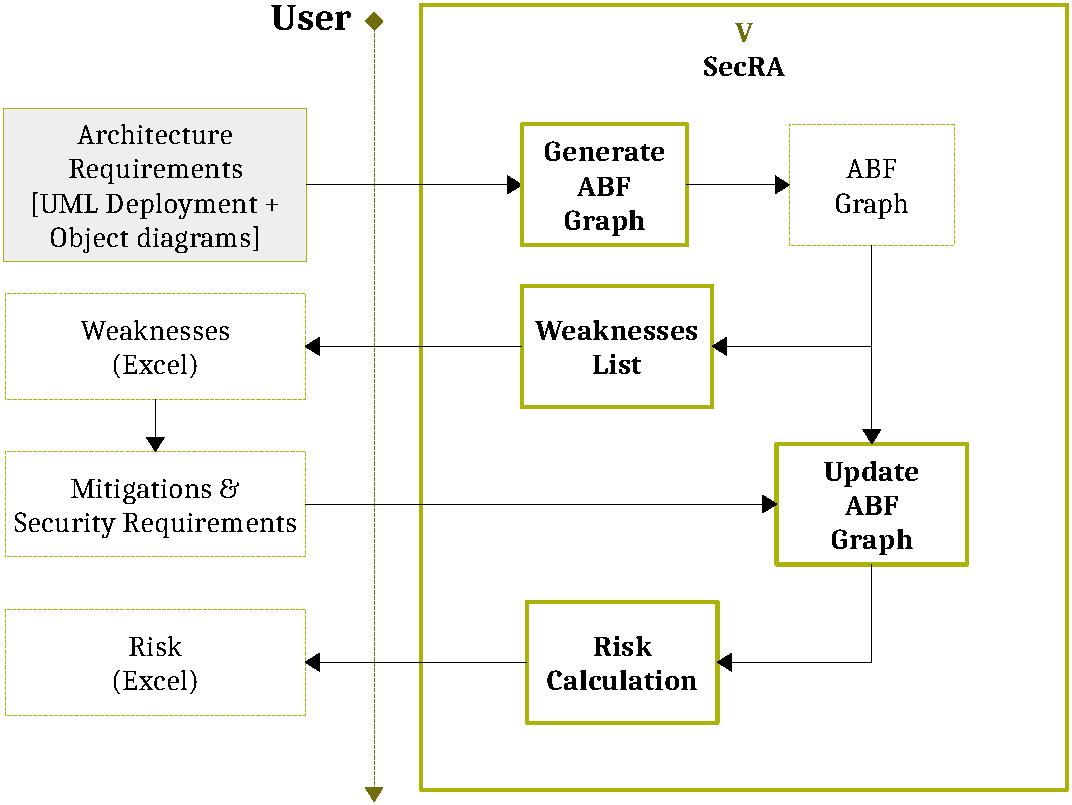
\includegraphics[width=.5\columnwidth]{v-secra.pdf}
	\caption{Cybersecurity Risk Assessment Tool}
	\label{fig:secra}
\end{figure}
To test our hypothesis we implemented a tool-chain (open-source with
AGPLv3 license, available at \autocite{v-research2020cybersecurity}) for the
identification of weaknesses and the calculation of potential insecure
configurations. The engineering of the $\abftheory$-framework for CPS is summarized in the UML
Class diagram in Fig.~\ref{fig:secraclassdiagram} (in appendix). 
As in Fig.~\ref{fig:secra}, the cybersecurity risk assessment process
starts with the definition of the use cases and architectural requirements.  In our process, the specification is manually
translated into a UML design where:
\begin{itemize}
	\item A \emph{deployment diagram} describes the \emph{physical
		architecture}. Each agent is defined as an UML node with (physical)
		ports, and agent's ports are connected via UML information flow
		connectors, representing the physical channel.
	\item A \emph{functional architecture} is linked to each agent in the
		deployment diagram and is defined by an \emph{object diagram}.
		The object diagram is composed by instances of functional
		blocks, connected via information flow connectors.
	\item The connection between the two diagrams is implemented by
		``sockets'', functional blocks connected to a 
		physical port.
\end{itemize}

The tool generates a graph-like structure which represents
the specification ($\abftheory$-graph). The $\abftheory$-graph defines the system as
a number of regions of assertions, beliefs, and facts. Those regions
are connected by a generic relation which is evaluated as follows (according to
the formula in Section~\ref{sec:formula}).
The graph is translated into 
a logical formula that represents the specification in the $\abftheory$-framework and,
along with the axiomatization of the RCC5 calculus, is given as input to the Z3 SMT solver.
The solver identifies all possible configurations of the system and, in turn,
identifies all potential weaknesses. 
The $\abftheory$-graph can be viewed as PDF and the results are reported into an spreadsheet file.
The spreadsheet file also reports the total number of configurations as indicating
the cybersecurity risk associated to the specification. A user can change the status
of each weakness in the spreadsheet file from the default status (open)
to ``mitigated'' and the risk is re-calculated on-the-fly, i.e.
without the need of running the tool again, based on annotations and formulas 
in the spreadsheet file.
In our approach, cybersecurity requirements are not imposed by the
specification but are automatically extracted by our tool as mitigations to potential weaknesses,
which are related to the insecure configurations 
of the specified system. 


\paragraph{Case Study.}
\begin{figure}[t]
\begin{minipage}[t]{0.3\textwidth}
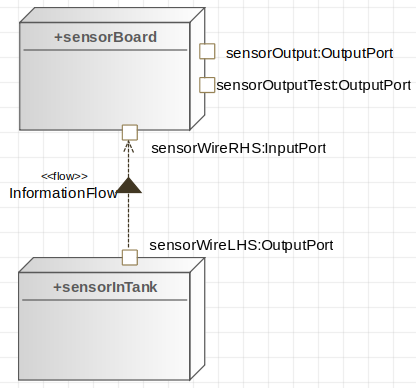
\includegraphics[width=\columnwidth]{eng_cs1.png}
\end{minipage}
\begin{minipage}[t]{0.7\textwidth}
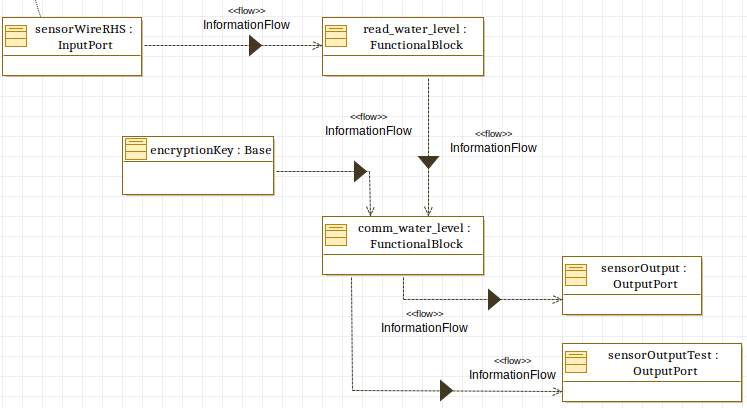
\includegraphics[width=\columnwidth]{internal_cs1.png}
\end{minipage}
  \caption{Sensor board object (left) and water level reader deployment (right) diagrams.}
\label{fig:int_cs1}
\label{fig:eng_cs1}
\end{figure}
We report here the results of the evaluation of a water level reader (sensor ad-hoc example). 
As in Fig.~\ref{fig:eng_cs1} (left), we defined 2 agents: sensorInTank and sensorBoard,
as the physical reader that needs to be placed in a tank, and 
the board that interprets the readings and outputs them as signals.
The two components are connected by a wire.
In Fig.~\ref{fig:int_cs1} (right), we report the functional architecture that
receives the incoming communications from the sensor in the tank and 
communicates them encrypted.
The tool (App.~\ref{app:results}) reports 16777216
scenarios in which at least one component diverge from the specification.

\section{Conclusion and Future Work}
We proposed a hypothesis for a foundational theory on security, arguing that
cybersecurity-related issues are not linked to the maliciousness of an agent
but to the vagueness in the design processes.  We provided a prototype
tool for the quantitative estimation of the cybersecurity risk based on a UML
model of a system.
The verification and test-case generation will be our next steps.

\printbibliography

\appendix
\section{Class Diagram for $\abftheory$-framework}
The Class Diagram for the Engineering of the $\abftheory$-framework is reported in
Fig.~\ref{fig:secraclassdiagram}. A \emph{specification} of a CPS is viewed
as an aggregation of \emph{architectures} which can describe the functional or
physical requirements. The physical components of the architecture are
input/output \emph{ports} and \emph{channels} (aggregations of pairs of ports)
while \emph{functional blocks} are the only constituents of the functional
architecture. All of the classes are abstract except input/output ports and
functional blocks. Therefore, agents (which represents sub-systems or
components) are composed by ports and functional blocks, as an aggregation of 
architectures.

\section{Overview of the Results of the Tool}\label{app:results}
In Fig.~\ref{fig:results} we show a screenshot of the 
results reported by our tool.
\begin{figure}[h]
	\centering
	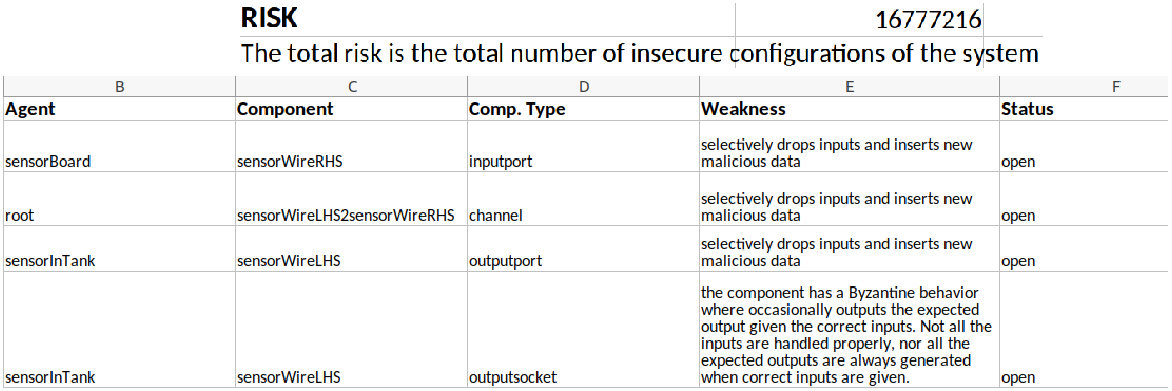
\includegraphics[width=\textwidth]{results.pdf}
	\caption{Partial View of the results in the spreadsheet file}
	\label{fig:results}
\end{figure}

\begin{sidewaysfigure*}
	\centering
	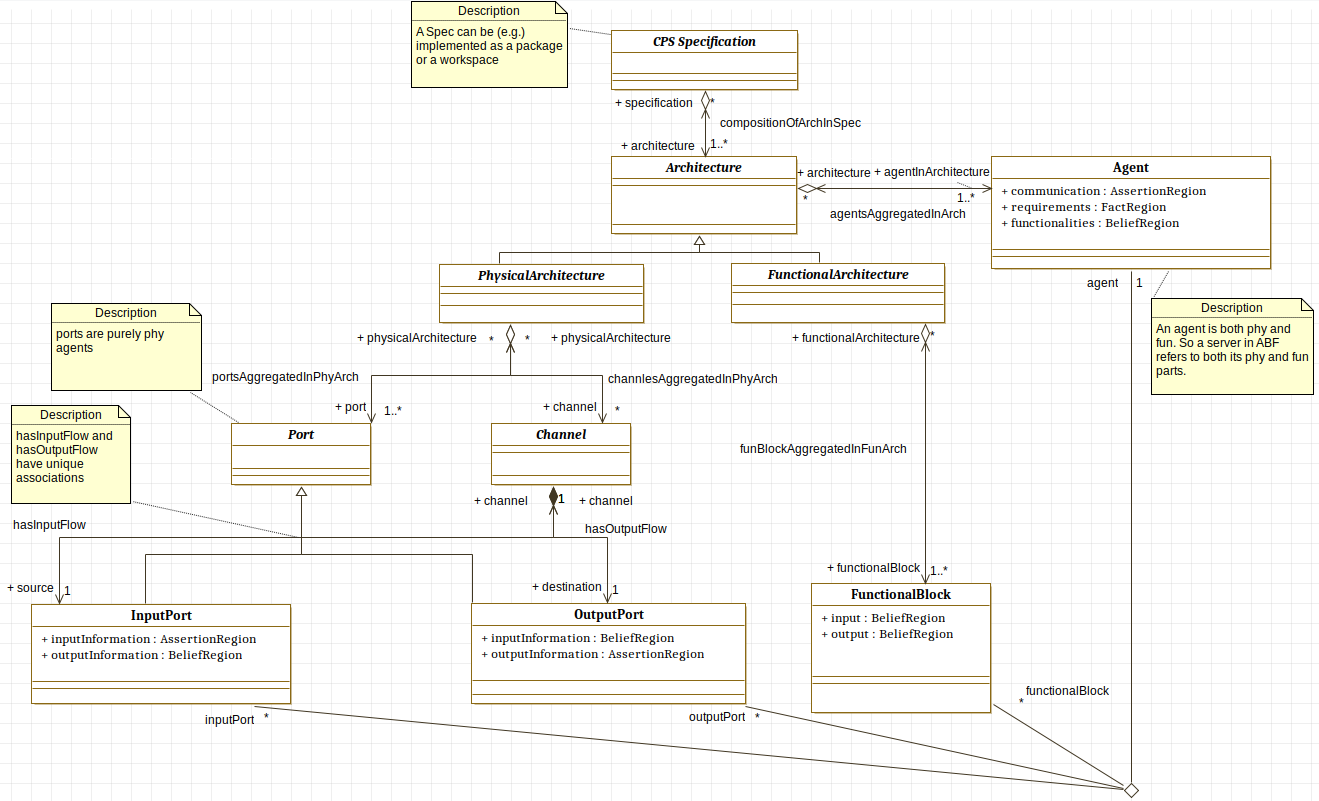
\includegraphics[width=\textwidth]{secra_classDiagram.png}
	\caption{$\abftheory$-framework for CPS Design -- Class Diagram}
	\label{fig:secraclassdiagram}
\end{sidewaysfigure*}



\end{document}
